\documentclass{hsflensburg}
\title{Bewegungserkennung auf mobilen Geräten mit Verwendung von GANs für eine automatische Datensatzgenerierung}
\subtitle{Master-Thesis}

\author{
  \name{Florian Hansen}\\
  \institution{Hochschule Flensburg}
}

\usepackage[ngerman]{babel}
\usepackage{csquotes}
\usepackage{biblatex}
\usepackage{amsmath}
\usepackage{amssymb}
\usepackage{mathtools}
\addbibresource{bibliography.bib}

\newtheorem{definition}{Definition}

\setcapindent{0pt}

\begin{document}
  \maketitle
  \tableofcontents

  \chapter{Einleitung}

  \chapter{Grundlagen}
  \section{Kullback-Leibler-Divergenz}
  Die Kullback-Leibler-Divergenz (KL-Divergenz) misst, wie sehr sich zwei
  Verteilungen voneinander unterscheiden und hat seinen Ursprung in der
  Informationstheorie. 
  \begin{definition}[Kullback-Leibler-Divergenz \cite{arjovsky2017wasserstein}]
    Seien $P$ und $Q$ zwei Wahrscheinlichkeitsfunktionen über den gleichen
    Wahrscheinlichkeitsraum $X$. Dann ist der Abstand bzw. die Divergenz der
    beiden Verteilungen definiert als
    \[
      D_{KL}(P \lvert\lvert Q) = \sum_{x \in X} P(x) \log \frac{P(x)}{Q(x)}.
    \]
  \end{definition}
  Dabei gibt $P \lvert\lvert Q$ eine Divergenz von der Ausgangsverteilung $P$
  zur Zielverteilung $Q$ an. Das Messen der Divergenz zwischen zwei
  Wahrscheinlichkeitsverteilungen findet insbesondere im Machine-Learning statt,
  um künstliche neuronale Netze und ihre Gewichte zu trainieren. Deshalb kann
  die KL-Divergenz auch als Loss-Funktion verwendet werden. Bemerkenswert ist
  hierbei, dass die KL-Divergenz asymmetrisch ist, also $D_{KL}(P \lvert\lvert
  Q) \neq D_{KL}(Q \lvert\lvert P)$. Die Distanz zwischen zwei Verteilungen
  unterscheidet sich demnach je nach Ausgangsverteilung.

  \section{Jensen-Shannon-Divergenz}
  \begin{definition}[Jensen-Shannon-Divergenz \cite{arjovsky2017wasserstein}]
    Seien $P$ und $Q$ zwei Wahr\-schein\-lichkeitsfunktionen über den gleichen
    Wahrscheinlichkeitsraum $X$. Dann ist die Jensen-Shannon-Divergenz der
    beiden Verteilungen definiert als
    \[
      D_{JS}(P \lvert\lvert Q) = \frac{1}{2} D_{KL}(P \lvert\lvert M) + \frac{1}{2} D_{KL}(Q \lvert\lvert M) \quad\quad \text{mit} \;\; M = \frac{1}{2}(P + Q)
    \]
  \end{definition}
  Die Jensen-Shannon-Divergenz kann als Erweiterung der
  Kullback-Leibler-Divergenz angesehen werden. Im Gegensatz zur
  Kullback-Leibler-Divergenz ist die Jensen-Shannon-Divergenz (JS-Divergenz)
  symmetrisch. Das bedeutet, dass der Abstand zwischen zwei
  Wahrscheinlichkeitsverteilungen gleich groß ist, egal von welchen er beiden
  Distributionen aus betrachtet wird.

  \section{Wasserstein-Abstand}

  \chapter{Generative Adversarial Networks}
  In Machine-Learning existieren viele verschiedene Modelle, die vorhandene
  Datensätze analysieren und anhand der Daten lernen, Strukturen in den
  Datensätzen zu erkennen.  Besitzt man beispielsweise einen Datensatz
  bestehend aus Fotoaufnahmen von Tieren, so kann ein Klassifizierer trainiert
  werden, um einem Bild eine Tierklasse zuzuweisen. Aus diesem Grund fässt man
  diese Modelle unter dem Begriff \textit{Bildklassifizierung} zusammen.

  Wesentlich interessanter ist das Erkennen von vielen Objekten innerhalb eines
  Bildes, anstatt das gesamte Bild nur einer einzigen Klasse zuzuweisen. In der
  \textit{Objekterkennung} entwickelt man Modelle, welche mehr als nur eine
  Klasse erkennen können. Sie liefern zusätzlich zu den erkannten Klassen ihre
  Position und Größe innerhalb des Bildes. Diese Modelle treffen also keine
  Aussage über das Gesamtbild, sondern treffen Aussagen über einzelne Objekte
  innerhalb des Bildes.

  Neben Modellen, die zu einem bestimmten Sachverhalt eine Aussage treffen
  können, existieren auch Modelle, welche in der Lage sind, neue Sachverhalte zu
  erzeugen. Diese fallen unter dem Begriff \textit{Generative Adversarial
  Networks} (GANs) und bilden das Hauptthema dieses Abschnitts. Das interessante
  an diesen generativen Modellen ist, dass sie nicht nur die Strukturen eines
  Datensatzes lernen, sondern darüber hinaus neue Elemente der
  Ausgangsdistribution erzeugen können. Trainiert man also ein generatives
  Modell auf einen Datensatz, welcher Bilder von verschiedenen Tieren enthält,
  können neue Bilder der gleichen Art erzeugt werden.
  
  Aber nicht nur zum Erzeugen von Bildern kann diese Art von Modellen verwendet
  werden. Auch bei Aufgaben, bei denen eine Voraussagung getroffen werden soll,
  werden generative Modelle eingesetzt. Beispielsweise wurde in
  \cite{barsoum2017hpgan} gezeigt, wie zu bereits getätigten menschlichen
  Bewegungen unterschiedliche, darauf folgende Bewegungssequenzen aussehen
  können. Hier hat man also versucht, eine Vorhersage zur Entwicklung von
  menschlichen Bewegung zu tätigen.

  Die Funktionsweise von GANs ist im Prinzip ziemlich simpel. Während beim
  klassischen supervised-learning in der Regel nur ein Modell beim Training
  involviert ist, verhält sich das bei generativen Modellen etwas anders. Zum
  Einen wird ein Generator definiert, welcher, wie sein Name andeutet, Ausgaben
  selbst erzeugt. Zum Anderen wird ein Diskriminator in das Training eingebaut,
  welcher zwischen künstlich erzeugten und reellen Daten unterscheidet. Diese
  beiden Modelle werden dann gleichermaßen trainiert. Während der Generator
  versucht, Fälschungen immer genauer zu erzeugen, versucht der Diskriminator
  immer besser zwischen Fälschung und Realität zu unterscheiden. Die
  Ausgabe des Diskriminators ist dementsprechend entweder 0 für Fälschung und 1
  für Realität. Mit anderen Worten, die beiden Komponenten spielen Spiel, in
  welchem die eine Partei versucht, die andere zu täuschen
  \cite{goodfellow2014generative}.

  \[
    \min_G \max_D V(G, D) = \mathbb{E}_{x \sim p_{data}(x)}\left[ \log D(x) \right] + \mathbb{E}_{z \sim p_z(z)}\left[ \log (1 - D(G(z))) \right]
  \]

  Im Verlauf des Trainings entwickelt sich damit ein Generator, welcher im
  Idealfall so gute Fälschungen erzeugt, sodass sich diese nicht mehr von Daten
  der Ausgangsdistribution unterscheiden lassen. Der Diskriminator kann hier
  bestenfalls nur raten, kann also eine Genauigkeit von höchstens 50\%
  erreichen. Ist dies nicht der Fall, d.h. der Diskriminator kann Fälschungen
  mit einer höheren Wahrscheinlichkeit von realen Daten unterscheiden, so
  entsteht ein Ungleichgewicht. Aus diesem Grund sollten die Lernparameter
  sorgfältig ausgewählt und untersucht werden, damit ein stabil laufendes GAN
  trainiert wird.
  
  \section{Das Mode-Collapse-Problem}
  Ein großes Problem beim Trainieren von generativen neuronalen Netzen ist, dass
  sich der Generator sehr häufig auf bestimmte Merkmale der Ausgangsdistribution
  des Datensatzes fixiert. Das Ergebnis sind signifikant erhöht wiederkehrende
  Ergebnisse, die sich kaum bis gar nicht von anderen Ausgaben unterscheiden.
  Man erwartet jedoch, dass das jeweilge GAN eine vielseitige Variation aus
  allen Elementen des Datensatzes erzeugt. Mit anderen Worten, bei einer
  zufälligen Eingabe in das Netz, soll immer eine unterschiedliche Ausgabe
  erzeugt werden. Bei einem Mode-Collapse ist dies nicht der Fall. Es kann
  beispielsweise passieren, dass wenn das Netz auf das Erzeugen von neuen
  Gesichtern trainiert wird, dass dieses ausschließlich weibliche Gesichter
  erzeugt, weil das Netz herausgefunden hat, dass es einfacher ist, weibliche
  Gesichtszüge zu generieren, als männliche \cite{richardson2018gans}. Dies
  lässt sich damit erklären, dass der Generator beim Trainingsvorgang mehr
  Erfolg beim Generieren von weiblichen Gesichtern hatte und der Diskriminator
  es schwerer hatte, Fälschung von Realität zu unterscheiden. Um das Problem zu
  beseitigen wurden einige Erweiterungen an dem Standardmodell des GAN von
  \cite{goodfellow2014generative} hinzugefügt.

  \section{Deep Convolution GAN}
  Das \textit{Deep Convolution GAN} (DCGAN) ist ein Versuch,
  \textit{Convolutional Neural Networks} (CNNs) mit GANs zu verküpfen. Nach
  vielen Fehlschlägen in der Entwicklung von GANs mit CNNs ist die Version von
  \cite{radford2016unsupervised} stabil und auf viele unterschiedliche
  Datensätze anwendbar. Dafür wurden viele verschiedene Kombinationen von
  Schichten untersucht und es wurde dabei eine Architektur ausgearbeitet, die
  in ein stabiles Training über verschiedenste Datensätze resultierte.
  Zusätzlich können mithilfe dieser Architektur höherere Auflösungen und tiefere
  Netze erreicht werden.

  Zusätzlich zur eigentlichen Architektur von DCGAN werden moderne Techniken
  verwendet, um CNN-Architekturen zu vereinfachen.  Damit der Generator über
  mehrere Schichten hinweg die räumliche Darstellung von Objekten lernen kann,
  werden Convolutional-Layer verwendet. Anstatt, dass sogenannte
  Max-Pooling-Layer zum Einsatz kommen, können nach
  \cite{springenberg2015striving} einfach Convolutional-Layer mit erhöhtem
  Stride verwendet werden, ohne dass die Genauigkeit sinkt. In Bezug zu DCGANs
  von \cite{radford2016unsupervised} werden solche Schichten verwendet, um dem
  Generator das Erlernen vom räumlichen Upsampling zu ermöglichen. Auch der
  Diskriminator wird mit solchen CNN-Layer ausgestattet, um räumliches
  Downsampling zu erlernen.

  Neben dem Auslassen von Max-Pooling-Layer folgt DCGAN auch dem Trend,
  Fully-Connected-Layer vor jedem Convolutional-Feature zu vermeiden. Dabei
  wurde festgestellt, dass die Verknüpfung von Fully-Connected-Layer und der
  Eingabe des Generators bzw. mit der Ausgabe des Diskriminators am besten
  funktionieren. Die erste Schicht des Generators ist also ein
  Fully-Connected-Layer (1-dimensional), jedoch wird die Ausgabe der Schicht in
  einen 4-dimensionalen Tensor umgewandelt. Im Falle des Diskriminators wird die
  Ausgabe des letzen Convolutional-Layers (4-dimensional) abgeflacht und in eine
  1-dimensionale Schicht mit einer Sigmoid-Aktivierungsfuntion gefüttert
  \cite{radford2016unsupervised}.

  Um Mode-Collapse zu vermeiden, verwendet \cite{radford2016unsupervised}
  Batch-Normalization-Layer. Dadurch wird das Training stabilisiert und Probleme
  wie \textit{Internal-Covariate-Shifting} angegangen \cite{pmlr-v37-ioffe15}.
  Vor allem wird dadurch aber auch verhindert, dass der Generator immer die
  gleichen Ausgaben erzeugt. Das Anwenden der Batch-Normalisierung in allen
  Schichten des Netzwerks führt jedoch zur Stichprobenoszillation und
  Instabilität des Modells. Aus diesem Grund wird auf Batch-Normalization in der
  Ausgabesschicht des Generators und in der Eingabeschicht des Diskriminators
  verzichtet.

  Als letzte Beobachtung stellt \cite{radford2016unsupervised} fest, dass das
  Hinzufügen von ReLU-Ak\-ti\-vier\-ungs\-funk\-tio\-nen in allen Schichten des
  Generators zu schnellerem Lernen und Abdeckung der Farbräume der
  Trainingsdistribution führt. In der Ausgabeschicht wird jedoch anstatt von
  ReLU-Aktivierung eine Tanh-Aktivierung verwendet. Innerhalb des Diskriminators
  werden schließlich Leaky-ReLU-Aktivierungen angewandt.

  \begin{figure}
    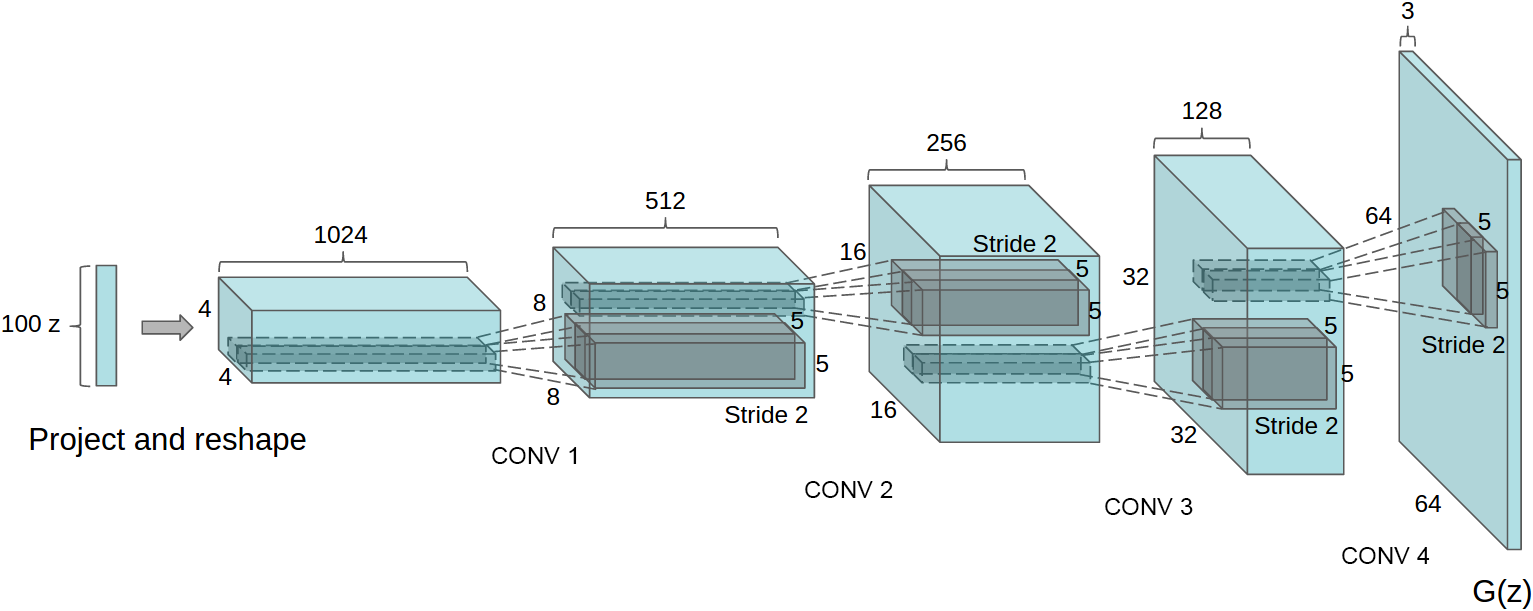
\includegraphics[width=\textwidth]{images/dcgan-architecture}
    \caption{DCGAN-Architektur des Generators von
    \cite{radford2016unsupervised}. Als Eingabe dient ein 100-dimensionaler
    Vektor, dessen Elemente zufällig gewählt werden. Dieser wird dann in den
    ersten Schichten umgeformt und durch vier Convolutional-Layer auf die Form
    3$\times$64$\times$64 gebracht. Die Strides geben dabei den
    Vergrößerungsfaktor pro Convolution-Schicht an, während die Anzahl der
    Filter den Farbkanälen entsprechen.}
  \end{figure}

  \section{Wasserstein GAN}
  \section{Wasserstein GAN mit Gradient Penality}

  \chapter{Erstellen eines Datensatzes}
  \section{Rahmenbedingungen}
  \section{Verwendung von GANs}
  \section{Durchführung von Experimenten mit unterschiedlichen GANs}
  \section{Analyse der Ergebnisse aus den Experimenten}

  \chapter{Bewegungserkennung}
  \section{Ground-Truth}
  \section{Background-Substraction}
  \section{Erkennung von Geschwindigkeiten}
  \section{Erkennung von Anomalien}
  \section{Erkennung von Bewegungsarten}
  \section{Vorhersage von Bewegungen}
  \section{Architektur einer mobilen Anwendung}

  \chapter{Fazit und Ausblick}

  \printbibliography
\end{document}
